\documentclass{beamer}
\usepackage[utf8]{inputenc}
\usetheme{Madrid}
\usecolortheme{default}
\usepackage{amsmath,amssymb,amsfonts,amsthm}
\usepackage{txfonts}
\usepackage{tkz-euclide}
\usepackage{listings}
\usepackage{adjustbox}
\usepackage{array}
\usepackage{tabularx}
\usepackage{gvv}
\usepackage{lmodern}
\usepackage{circuitikz}
\usepackage{tikz}
\usepackage{graphicx}

\setbeamertemplate{page number in head/foot}[totalframenumber]

\usepackage{tcolorbox}
\tcbuselibrary{minted,breakable,xparse,skins}
\definecolor{bg}{gray}{0.95}
\DeclareTCBListing{mintedbox}{O{}m!O{}}{%
  breakable=true,
  listing engine=minted,
  listing only,
  minted language=#2,
  minted style=default,
  minted options={%
    linenos,
    gobble=0,
    breaklines=true,
    breakafter=,,
    fontsize=\small,
    numbersep=8pt,
    #1},
  boxsep=0pt,
  left skip=0pt,
  right skip=0pt,
  left=25pt,
  right=0pt,
  top=3pt,
  bottom=3pt,
  arc=5pt,
  leftrule=0pt,
  rightrule=0pt,
  bottomrule=2pt,
  toprule=2pt,
  colback=bg,
  colframe=orange!70,
  enhanced,
  overlay={%
    \begin{tcbclipinterior}
    \fill[orange!20!white] (frame.south west) rectangle ([xshift=20pt]frame.north west);
    \end{tcbclipinterior}},
  #3,
}
\lstset{
    language=C,
    basicstyle=\ttfamily\small,
    keywordstyle=\color{blue},
    stringstyle=\color{orange},
    commentstyle=\color{green!60!black},
    numbers=left,
    numberstyle=\tiny\color{gray},
    breaklines=true,
    showstringspaces=false,
}
\begin{document}

\title 
{5.9.14}
\date{september 15,2025}


\author 
{Namaswi-EE25BTECH11060}
\frame{\titlepage}
\begin{frame}{Question}On her birthday Seema decided to donate some money to children of an orphanage home. If there were 8 children less, every one would have got  10 Rupees more. However,if there were 16 children more, every one would have got  10 Rupees less. Using matrix method, find the number of children and the amount distributed by Seema. What values are reflected by Seemas decision ?
\end{frame}
\begin{frame}{Theoritical Solution}
    Let, Number of children=c and Amount=a\\
Given,\\
\begin{align}
   ca=(c-8)(a+10)=(c+16)(a-10) 
\end{align}
From 1,
\begin{align}
    10c-8a=80\\
    10c-16a=-160
\end{align}
\end{frame}
\begin{frame}{Solution}
   From 2,
\begin{align}
    \begin{pmatrix}
        5 \\ -4
    \end{pmatrix}^\top \begin{pmatrix}
        c \\ a
    \end{pmatrix}=40
    \end{align}
    From 3,
\begin{align}
    \begin{pmatrix}
     5  \\ -8   
    \end{pmatrix}^\top \begin{pmatrix}
        c \\ a
    \end{pmatrix}=-80\\
    \begin{pmatrix}
        5 & -4 \\
        5 & -8
    \end{pmatrix}\begin{pmatrix}
        c \\ a
    \end{pmatrix}=\begin{pmatrix}
        40 \\ -80
    \end{pmatrix}
\end{align} 
\end{frame}
\begin{frame}{Solution}
   Forming argumented matrix
\begin{align}
    \augvec{2}{1}{5 & -4 & 40 \\ 5 & -8 & -80}
\end{align}
Replace
\[R_2 \to R_2-R_1\]
\begin{align}
\augvec{2}{1}{5 & -4 & 40 \\ 0 & -4 & -120} 
    \end{align}
Replace
\[R_2 \to R_2/-4\]
\begin{align}
      \augvec{2}{1}{5 & -4 & 40 \\ 0 & 1 & 30} 
\end{align}
\end{frame}\begin{frame}{Solution}
    Replace 
\[R_1 \to R_1+4R_2\]
\begin{align}
    \augvec{2}{1}{5 & 0 & 160 \\ 0 & 1 & 30} 
\end{align} 
Replace
\[R_1 \to R_1/5\]
\begin{align}
      \augvec{2}{1}{1 & 0 & 32 \\ 0 & 1 & 30} 
\end{align}
so,
\begin{align}
    c=32 \quad  a=30
\end{align}
\end{frame}
\begin{frame}[fragile]
\frametitle{C Code}
\begin{lstlisting}
    #include <stdio.h>
int main() {
    double mat[2][3] = {
        {5, -4, 40},
        {5, -8, -80}
    };

    for (int j = 0; j < 3; j++) {
        mat[1][j] = mat[1][j] - mat[0][j];
    }
    for (int j = 0; j < 3; j++) {
        mat[1][j] = mat[1][j] / -4;
    } 
\end{lstlisting}
\end{frame}
\begin{frame}[fragile]
\frametitle{C Code}
\begin{lstlisting}
     for (int j = 0; j < 3; j++) {
        mat[0][j] = mat[0][j] + 4 * mat[1][j];
    }
    for (int j = 0; j < 3; j++) {
        mat[0][j] = mat[0][j] / 5;
    }
    // Solution
    double c = mat[0][2];
    double a = mat[1][2];
    printf("Solution:\n");
    printf("Number of children (c) = %.0f\n", c);
    printf("Amount (a) = %.0f\n", a);
    return 0;
}
\end{lstlisting}
\end{frame}
\begin{frame}[fragile]
\frametitle{Python Code}
\begin{lstlisting}
    import numpy as np
import matplotlib.pyplot as plt
# Define the lines as functions: m = f(c)
# Line 1: 5c - 4m = 40  -> m = (5c - 40)/4
# Line 2: 5c - 8m = -80 -> m = (5c + 80)/8

# Choose range for c
c = np.linspace(-20, 20, 400)

# Compute m for both lines
m1 = (5*c - 40)/4
m2 = (5*c + 80)/8
\end{lstlisting}
\end{frame}
\begin{frame}[fragile]
\frametitle{Python Code}
\begin{lstlisting}
    # Plot the lines
plt.plot(c, m1, label=r'$5c - 4m = 40$', color='blue')
plt.plot(c, m2, label=r'$5c - 8m = -80$', color='red')

# Labels and title
plt.xlabel('c')
plt.ylabel('m')
plt.title('Graph of Two Lines')
plt.grid(True)
plt.legend()

# Show plot
plt.show()
\end{lstlisting}
\end{frame}
\begin{frame}[fragile]
\frametitle{C and Python Code}
\begin{lstlisting}
    import ctypes
# Load the shared library
lib = ctypes.CDLL("./gauss_solver.so")
# Prepare C variables
c = ctypes.c_double()
a = ctypes.c_double()

# Call the function
lib.solve_system(ctypes.byref(c), ctypes.byref(a))

print(f"Number of children (c) = {c.value}")
print(f"Amount (a) = {a.value}")
\end{lstlisting}
\end{frame}
\begin{frame}{plot}
\begin{align}
\centering
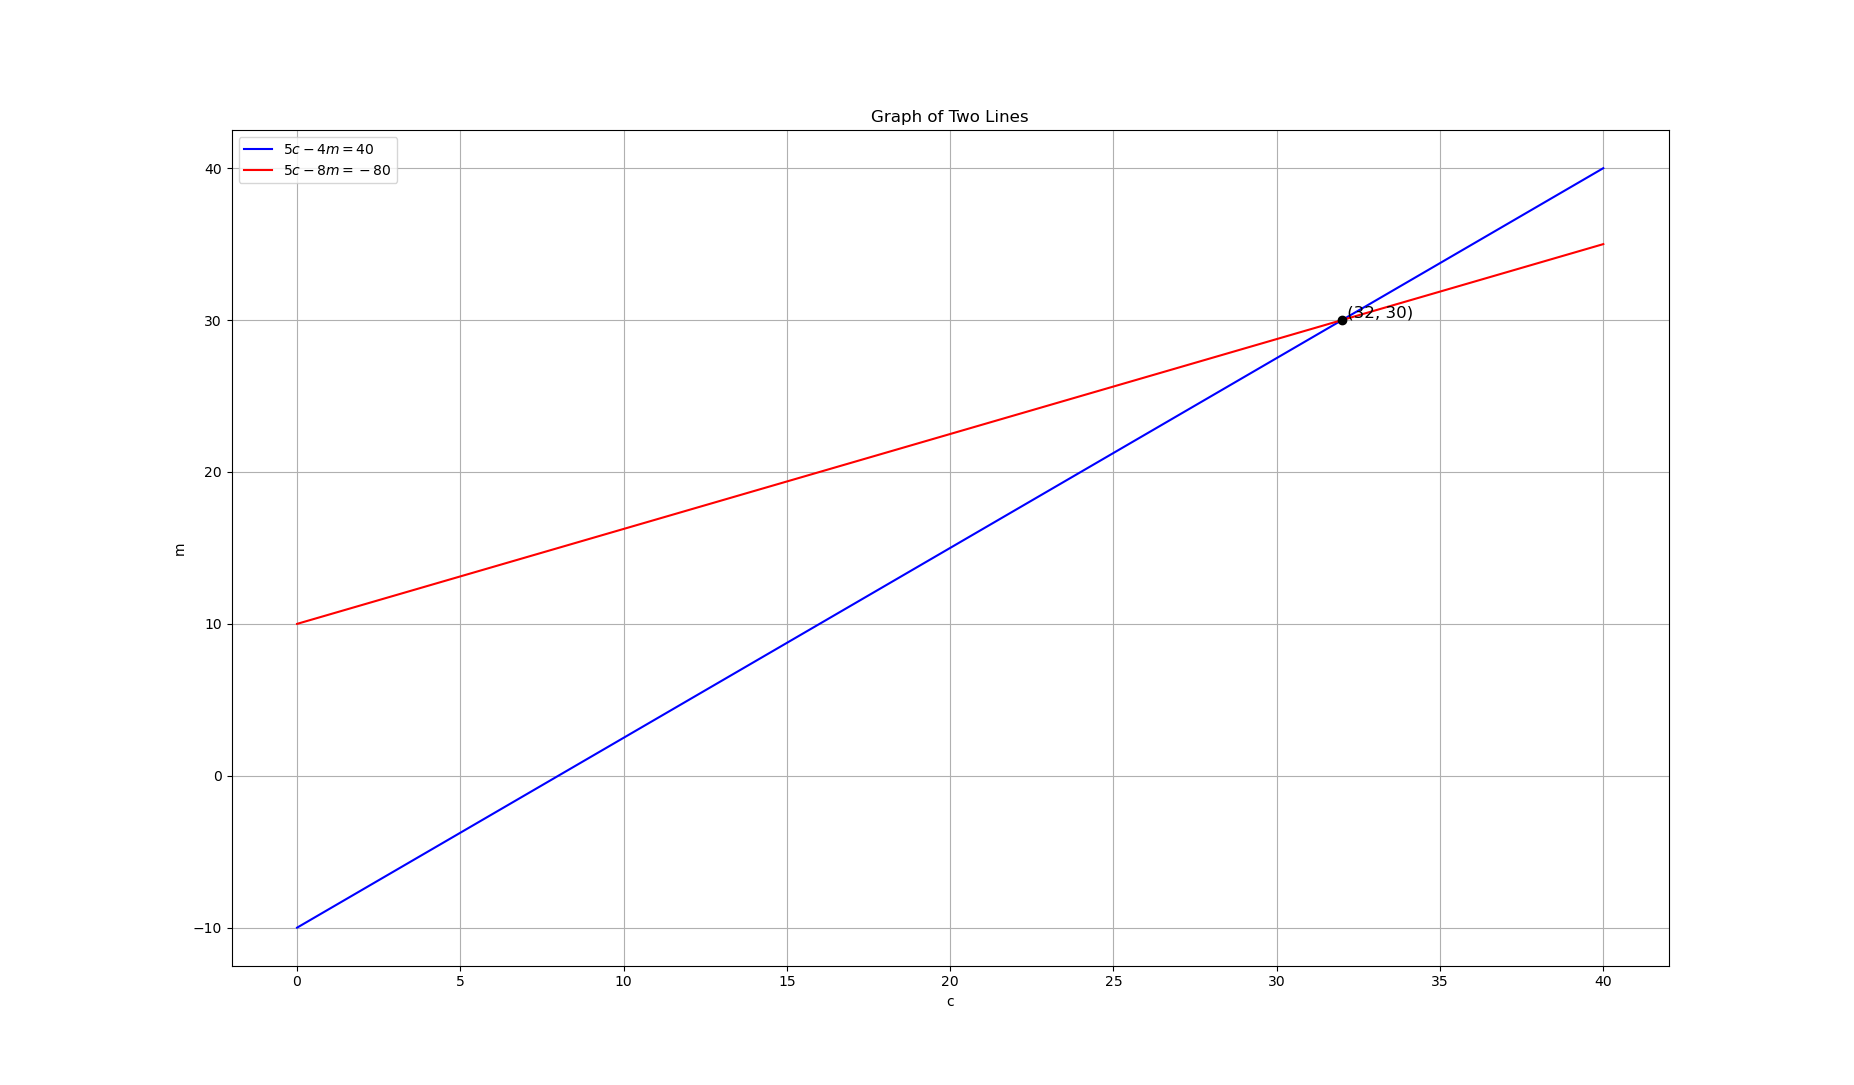
\includegraphics[width=\columnwidth, height=0.8\textheight, keepaspectratio]{Figure_12 .png}   
\end{align}
    
\end{frame}
\end{document}
